\documentclass[twocolumn,12pt,a4paper]{article}

\usepackage[english]{babel}
\usepackage[utf8]{inputenc}
\usepackage[T1]{fontenc}
\usepackage{multicol}
\usepackage[top=3cm, bottom=3cm, left=2.5cm, right=2.5cm]{geometry}
\usepackage[bookmarks=true,bookmarksnumbered=true,hidelinks]{hyperref}
\usepackage{fancyhdr,lastpage}
\renewcommand{\footrulewidth}{0.4pt}
\usepackage[bf,sf]{titlesec}
\usepackage{siunitx}
\usepackage{titling,graphicx}
\usepackage{abstract}
\usepackage{amsmath}
\usepackage{siunitx}

\pagestyle{fancy}
\lhead{\textsf{Solar Sailing from Earth to Mars}}
\rhead{\textsf{Team 891}}
\cfoot{\thepage{} of \pageref*{LastPage}}

\setlength{\columnsep}{1.5cm}

% Numerar equacions amb la secció
\numberwithin{equation}{section}

\author{\textsf{Team 891}}
\title{\textsf{\textbf{Problem A: Solar Sailing from Earth to Mars}}}
\date{\textsf{November 12, 2017}}

\begin{document}
\renewcommand{\abstractname}{}
\renewcommand{\absnamepos}{empty}
\begin{titlingpage}
 \maketitle

\noindent \hrulefill \\
\begin{abstract}
Test test test

\end{abstract}
\hrulefill \\

\end{titlingpage}

\clearpage

\section{Introduction}
\subsection{Restatement of the problem}

 A more detailed interpretation of the problem was needed so that a more precise model could be built. Understanding firstly the physical foundations around solar sailing was essential in order to perform an accurate analysis. Research has been done on the different forces affecting the sail for trajectories to be computed. Since some initial conditions are already given it has been necessary to verify whether these were the best options to accomplish the overall goal of the study or not.
 
  Moreover the aim of the survey is not only to calculate the path followed by the craft but also to determine its velocity so that a safe landing can be guaranteed. However, as trying to consider the attraction of Mars does not always give accurate results, this is not an easy task, though an estimate of craft arrival to Mars is presented at the end.
 
 It will be understood that the sail starts its trajectory with a radial velocity equal to the Earth's escape velocity, and with a tangential velocity equal to the Earth's linear velocity around the Sun. 
 
The release of the space craft will be considered at the time in which the Earth is closest to Mars, although, as it will be further discussed, results do not point in this being the best configuration. Since orbits of both planets are regarded as circular, as mentioned in the following section, this occurs when the Earth, Mars and the Sun are aligned.

The main goals of the article are to discuss a suitable distribuiton of the mass of the space craft, as well as to simulate possible trajectories and the arrival of the sail to Mars.

\subsection{Main assumptions}
Throughout the article, several assumptions have been made, both as interpretations of the problem and in order to facilitate the model. However, all assumptions are supported by literature, and all the approximations were found to be reasonable. We present the approximations and interpretations made.

\begin{itemize}
\item The orbits of Mars and the Earth are coplanar and perfectly circular.
\item The only forces acting on the sail during its flight are the gravitational force exerted by the Sun and the thrust given by the inciding photons. Since the initial radial velocity is the Earth escape velocity, it is reasonable not to consider its attraction. However, Mars gravitational pull has been taken into account when calculating the arriving velocity.
\item As stated in the problem given, we assume the total mass of the space craft is \SI{2 000}{kg} , including the payload and the sail. Thus, our goal is to maximize the payload while still finding a reasonable time of flight. 
\item Comparing the research which has already been done to the fact that the preassure exerted by light is twice its energy density, one finds that the case given is one of a perfect reflection.
\item We assume the only initial radial velocity of the sail is the Earth's linear velocity. Thus, one ignores the effects of the Earth's rotation.
\end{itemize}


\section{The physics of solar sailing}
We will follow \cite{tsu} and \cite{mcinnes} for most of this section.
\subsection{Radiation pressure}
It is well-known that electromagnetic wave carries an energy density. The fundamental idea behind solar sails is to use this energy as a means of propulsion in a way very much similar to how traditional sails take advantage of the kinetic energy of the wind. Given that the diameter of any reasonable solar sail will be much smaller than its distance to the Sun, one may approximate the solar radiation that arrives at the sail in the form of sinusoidal planar waves of frequency \( \omega \).

If \( E(t) \) is the amplitude of such waves, then the energy density, \( u \), they carry is given by \( u = \epsilon_0 E(t)^2 = \epsilon_0 E_0^2 \cos^2{\omega t} \). If one averages this over a period \( T \), then one obtains that the average energy density is simply \( \epsilon_0 E_0^2 /2 \), which can be rewritten as \( I/c \), where \( I \) is the intensity of the wave and \( c \) is the speed of light. Thus one finds that the pressure that incoming radiation exerts on the sail is \( I/c \). However, given that the material of the sail is not a black body, a fraction, \( R \), of the absorbed radiation will be emitted, giving rise to an additional term of pressure of the form \( RI/c \). If the sail is made out of a perfectly reflective material then it is the case that \( R = 1 \) and then the total pressure exerted on the sail is \( p = 2I/c \). This is the case for the problem at hand.

The intensity of a spherical wave is inversely proportional to the square of the distance from the source. Thus, the force exerted on the sail by the radiation from the Sun follows an inverse square law. We can make this dependence explicit by considering the equality \( Ir^2 = I_0 r^2_0 \), where \( I_0 \) is the intensity of solar radiation at a distance equal to the radius of the orbit of the Earth, \( r_0 \). And so we find that the force due to radiation pressure on a sail of surface area \( S \) is
\begin{equation}
 	\mathbf{F}_R(r) = \dfrac{2SI_0r_0^2}{c}\dfrac{1}{r^2} \mathbf{\hat{e}}_r \label{eq:radiation force}
\end{equation}

\subsection{Equations of motion for a solar sail: orthogonal case}
We have established that a solar sail that receives radiation in a direction orthogonal to itself experiences an inverse square central force. The other force acting on the sail is gravitational attraction due to the Sun ---we will consider the gravitational pull from other planets to be negligible when compared to that of the Sun---, which is also an inverse square force law. Namely:
\begin{equation}
 	\mathbf{F}_G(r) = -\dfrac{G M_S m}{r^2} \mathbf{\hat{e}}_r \label{eq:gravitational force}
\end{equation}
where \( m \) is the mass of the solar sail ---including the mass of the payload--- and \( M_S \) is the mass of the Sun.

Thus, we are now in a position to write the equations of motion for the solar sail
\begin{align}
	a_{r} &= \dot{v}_r - \dfrac{v_{\theta}^2}{r} = \dfrac{F_R - F_G}{m} \label{eq:equations of motion perpendicular} \\
	a_{\theta} &= \dot{v}_{\theta} + \dfrac{v_r v_{\theta}}{r} = 0 
\end{align}
It is common to introduce a number of parameters to better encapsulate the nature of a solar sail. The characteristic acceleration of a solar sail, \( a_R \), is defined to be the acceleration the sail experiences due to radiation pressure at a distance equal to 1 astronomical unit (AU) from the Sun. In keeping with the notation introduced in the previous section we write
\begin{equation}
  a_R = \dfrac{2SI_0}{mc}
\end{equation}
It is then immediate to see that, if we denote the acceleration due to radiation pressure by \( a_R \) we have
\begin{equation}
  a(r) = a_R \dfrac{r_0^2}{r^2} 
\end{equation}
We can do the same with the acceleration due to gravity and we find
\begin{equation}
  a(r) = a_G \dfrac{r_0^2}{r^2} = \dfrac{G M_s}{r_0^2} \dfrac{r_0^2}{r^2}
\end{equation}
With this in mind we can then rewrite \autoref{eq:equations of motion perpendicular} as follows
\begin{align} \label{eq:equations of motion characteristic accelerations}
  \dot{v}_r - \dfrac{v_{\theta}^2}{r} &= (a_R - a_G) \left(\dfrac{r_0}{r}\right)^2 \\
	\dot{v}_{\theta} + \dfrac{v_r v_{\theta}}{r} &= 0
\end{align}
As we have already mentioned, this shows that the motion of a solar sail receiving radiation orthogonal to itself is governed by an inverse square law. In particular, the sail will move as if it were orbiting a star with a mass less than the Sun.

\subsection{Equations of motion for a solar sail: general case}
This, however, is only true if the sail is orthogonal to the incoming radiation. Indeed, if we allow for the sail to be at an arbitrary orientation, then its tangential acceleration is no longer zero. For this, we introduce the angle \( \alpha \), which is the angle between the vector normal to the sail, \( \hat{\mathbf{n}} \), and the radial direction. Now, the force due to radiation pressure has two contributions. The incoming photons exert a force that is now proportional to the orthogonal projection of the sail onto the radial direction, therefore of \( IS\cos{\alpha}/c \). This force is in the radial direction. The emitted photons exert a force that has the same modulus, but given that the sail behaves like a mirror, they are emmited in the direction orthogonal to the radial direction, and so the force due to the outgoing radiation is proportional to \( {-\hat{\mathbf{e}}_{\theta}} \). So we have
\begin{equation}
  \mathbf{F}_R(r) = \dfrac{2IS \cos{\alpha}}{c} ( \hat{\mathbf{e}}_{r} - \hat{\mathbf{e}}_{\theta})
\end{equation}
We now observe that because of symmetry, the vector \( \hat{\mathbf{e}}_{r} - \hat{\mathbf{e}}_{\theta}  \) is proportional to \( \hat{\mathbf{n}} \), and, because \( \hat{\mathbf{n}} \) is a unit vector then we have \( \hat{\mathbf{e}}_{r} - \hat{\mathbf{e}}_{\theta} = \cos{\alpha} \hat{\mathbf{n}} \). 
And thus we obtain
\begin{align}
  \mathbf{F}_R(r) &= \dfrac{2IS \cos^2{\alpha}}{c} \hat{\mathbf{n}} \\
									&= \dfrac{2IS \cos^2{\alpha}}{c} (\cos{\alpha} \hat{\mathbf{e}}_r + \sin{\alpha} \hat{\mathbf{e}}_{\theta}) 
\end{align}

Finally, we can rewrite the equations of motion for a solar sail in this more general case as follows:
\begin{align}
  \dot{v}_r - \dfrac{v_{\theta}^2}{r} &= (a_R \cos^3{\alpha} - a_G) \left(\dfrac{r_0}{r}\right)^2\label{carlessexy} \\ 
  \dot{v}_{\theta} + \dfrac{v_r v_{\theta}}{r} &= -a_R	\sin{\alpha} \cos^2{\alpha} \left(\dfrac{r_0}{r}\right)^2
\end{align}
As a consistency check,  we note that if \( \alpha = 0 \), that is, the sail is orthogonal to the radiation, we recover \autoref{eq:equations of motion characteristic accelerations}. However, the equations we have just obtained are \emph{not} the equations for a particle experiencing central force motion.   

\section{First Results}
\subsection{The logarithmic spiral trajectory and discussion of a suitable distribuiton of mass}
According to what has been discussed in the previous section, there are some variables of the sail which have to be calculated. This are
\[
a_R=6,45\cdot 10^{-7} \cdot M_w
\]
\[a_G=5,928\cdot 10^{-3}
\]
where $M_w$ denotes the mass of the sail.
Another parameter
Literature suggests \cite{tsu} one can neglect the  $\dot{v}_r$ term in equation \ref{carlessexy} as a first approach. The simplified equation reads
\begin{equation}
- \dfrac{v_{\theta}^2}{r} = (a_R \cos^3{\alpha} - a_G) \left(\dfrac{r_0}{r}\right)^2
\end{equation} 
which can be directly solved.
Solving for $v_{\theta}$ and directly integrating, one can find the time of travel between radii $r_0$ and $r$.
\begin{equation}
	t=\frac{1}{3}\cdot\frac{r_0^{3/2}-r^{3/2}}{r_0\sqrt{a_R}}\cdot\frac{(a_G/a_R-\cos^3\alpha)^{1/2}}{\sin\alpha\cos^2\alpha}
\end{equation}
Thus, as a first approximation, the time of travel will be, substituting,
\[
Look it up
\]
Having solved both velocities, one finds the trajectory taken is a logarithmic spiral, which only depends on the ratio \(a_G/a_R\) and $\alpha$.
Figure ?? shows a first approximation of the trajectory taken by the space craft with the mentioned suppositions and values.

\begin{figure}
	\centering
	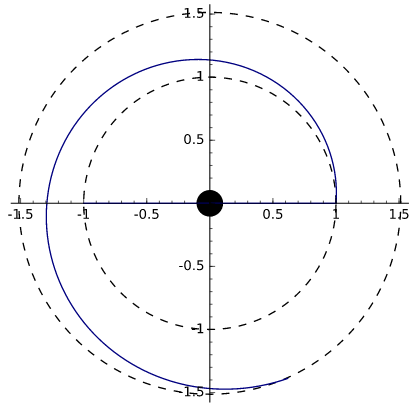
\includegraphics[scale=0.5]{espiral.png}
	\label{espiral}
	\caption{\small First approximation of the sail trajectory, in blue. The Sun is in the middle and the dashed lines represent the orbits of the Earth and Mars. Axis in AU.}
\end{figure}



\bibliographystyle{ieeetr}
\bibliography{UphysicscNotes}

\end{document}

